\appendix
% Delete the text and write Appendix here (not required, can be omitted):
% Comment out ' \appendix
% Delete the text and write Appendix here (not required, can be omitted):
% Comment out ' \appendix
% Delete the text and write Appendix here (not required, can be omitted):
% Comment out ' \appendix
% Delete the text and write Appendix here (not required, can be omitted):
% Comment out ' \input{Text/Appendix} ' to remove this section.
%------------------------------------


\section{Additional Information}
\subsection{Python codes}
All of the data processing and network trainings are done on Cats\_And\_Dogs.ipynb file. In \cref{listing:1} a basic implementation of cross validation can be seen. 
% because I have loaded varioref and cleveref (in that order) varioref has "become clever", and you can
% use \Vref{} in the start of a sentence.



\begin{listing}[!htb]

\inputminted[%
firstline=1, 
lastline=15,
bgcolor=LightGray,
breaklines,
breaksymbolleft={},
breakindent={15pt}
]{python}{Code/Python/kfold.py}

\caption{Basic K-Fold implementation}
\label{listing:1}
\end{listing}

The code from \cref{listing:1} was displayed using a \verb+.py+ file. Since the lines are not numbered in this code example, you can copy and paste the code from the PDF into python without many issues (does however need to correct indents). \par
The way cross folding that is implemented in the notebook is vastly different from what its written on here. This code is just an example for it.\par

\section{Model Summaries}
\begin{figure}
    \centering
    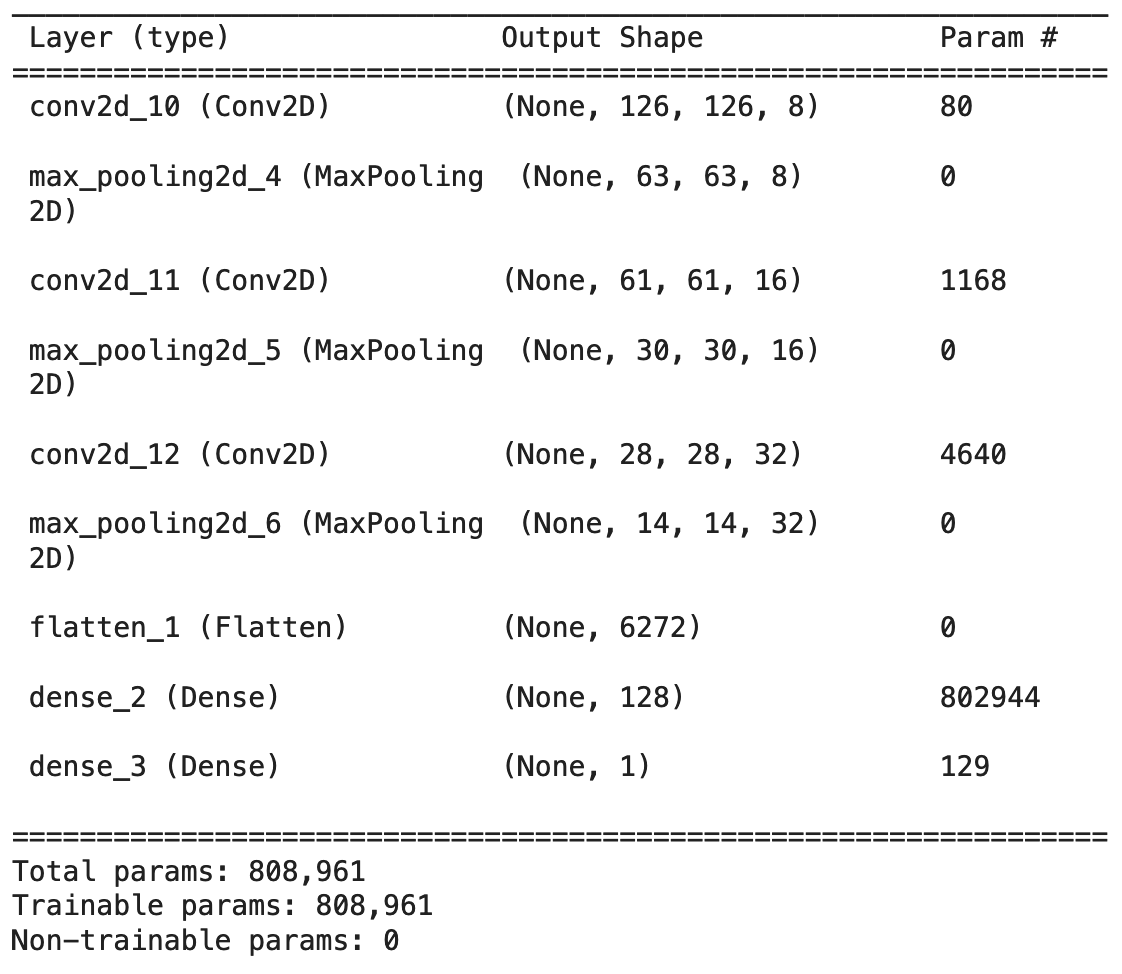
\includegraphics[width=0.48\textwidth]{Images/cnn_summary.png}
    \caption{CNN Summary}
    \label{fig:cnn_summary}
\end{figure}
\begin{figure}
    \centering
    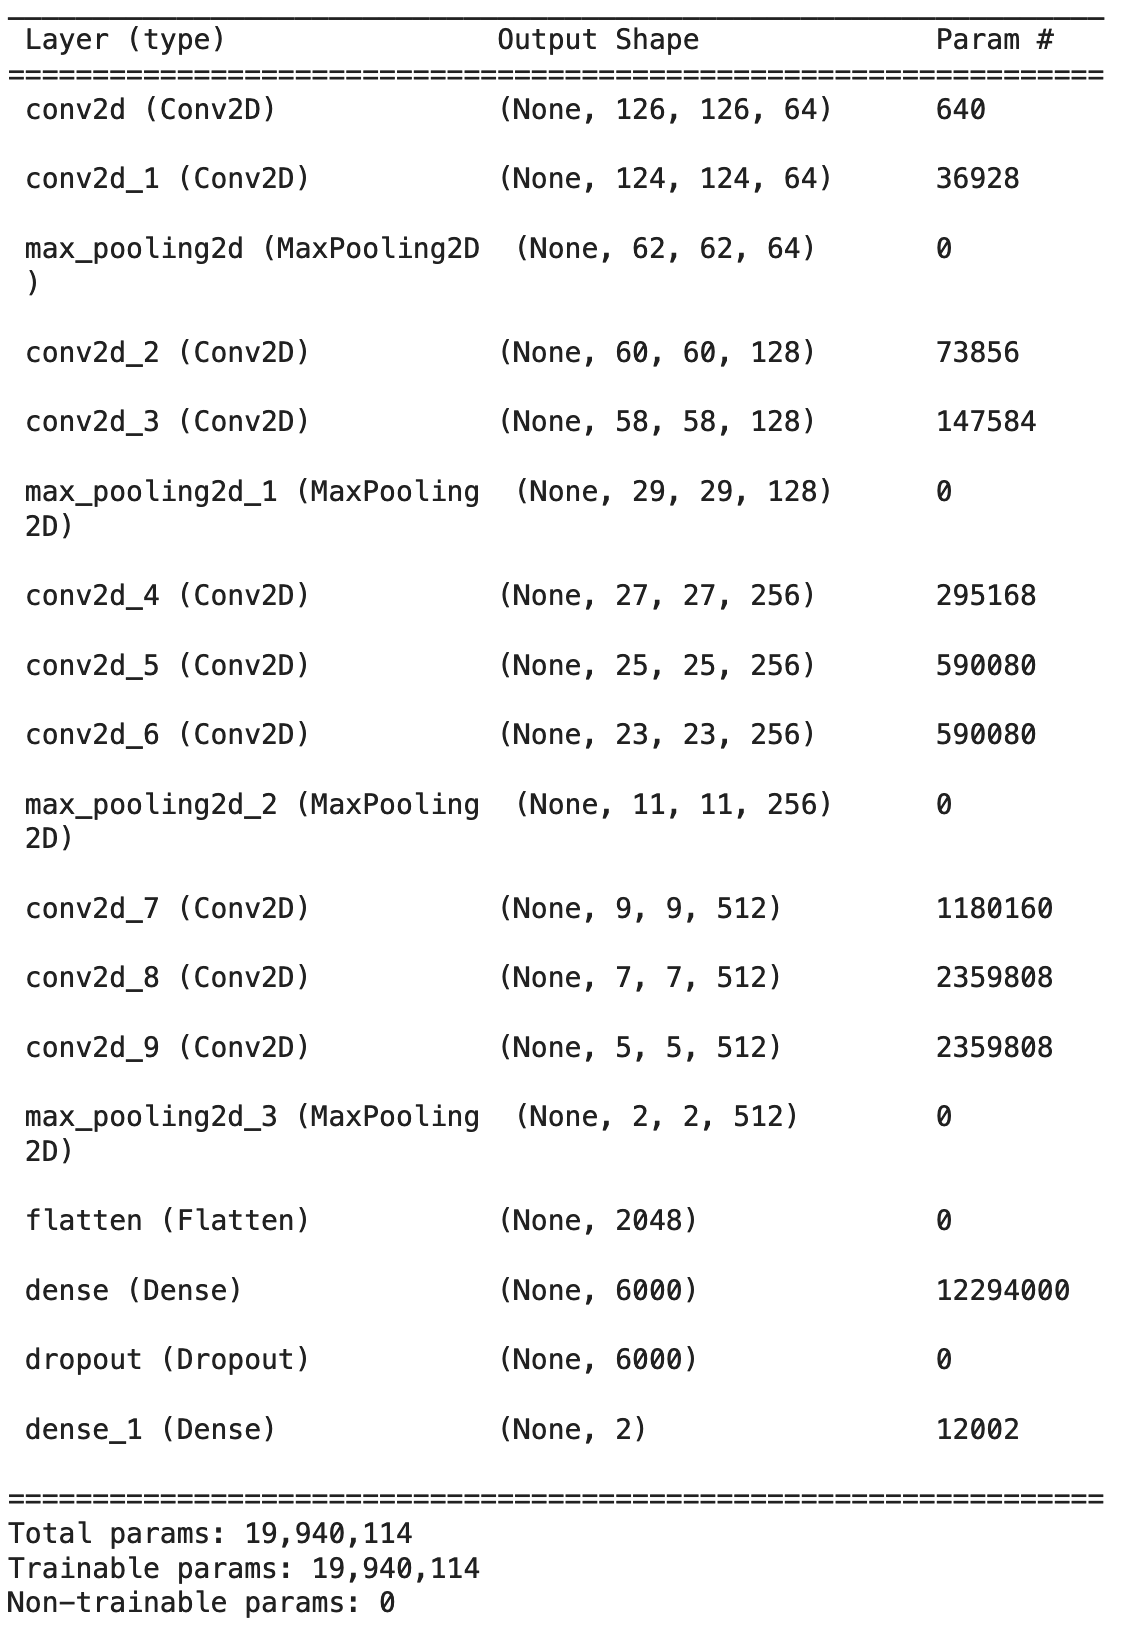
\includegraphics[width=0.48\textwidth]{Images/vgg13_summary.png}
    \caption{VGG13 Summary}
    \label{fig:vgg13_summary}
\end{figure}
\begin{figure}
    \centering
    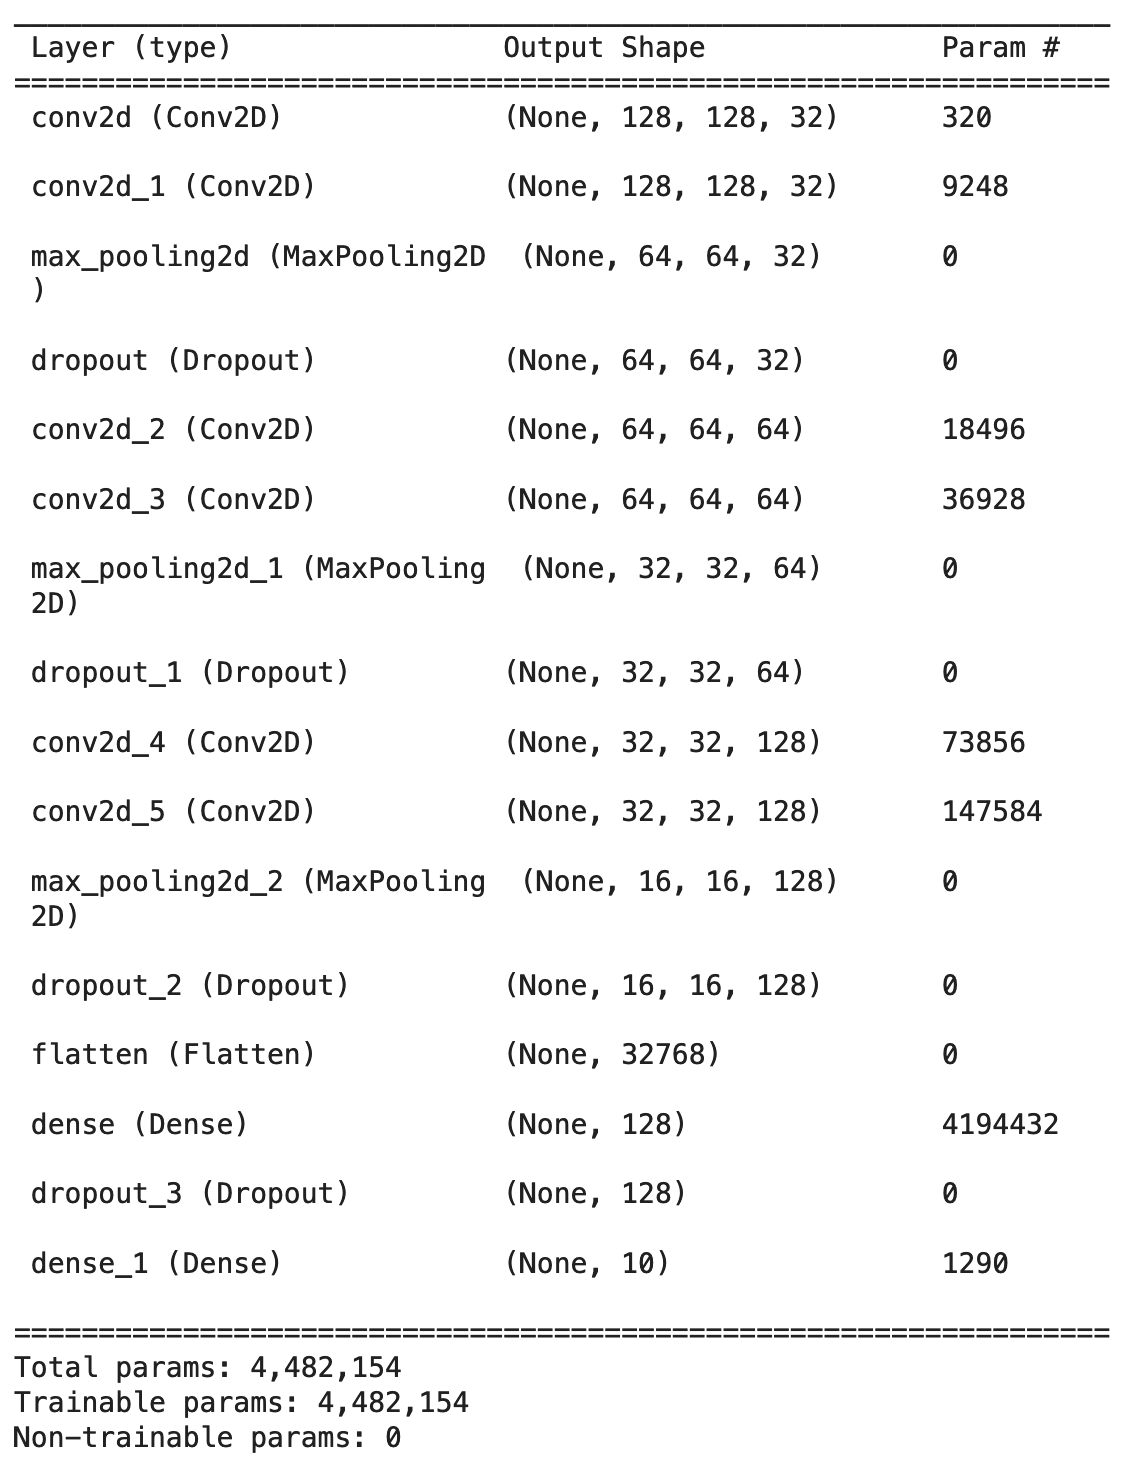
\includegraphics[width=0.48\textwidth]{Images/vgg3_summary.png}
    \caption{VGG3 Summary}
    \label{fig:vgg3_summary}
\end{figure}
\begin{figure}
    \centering
    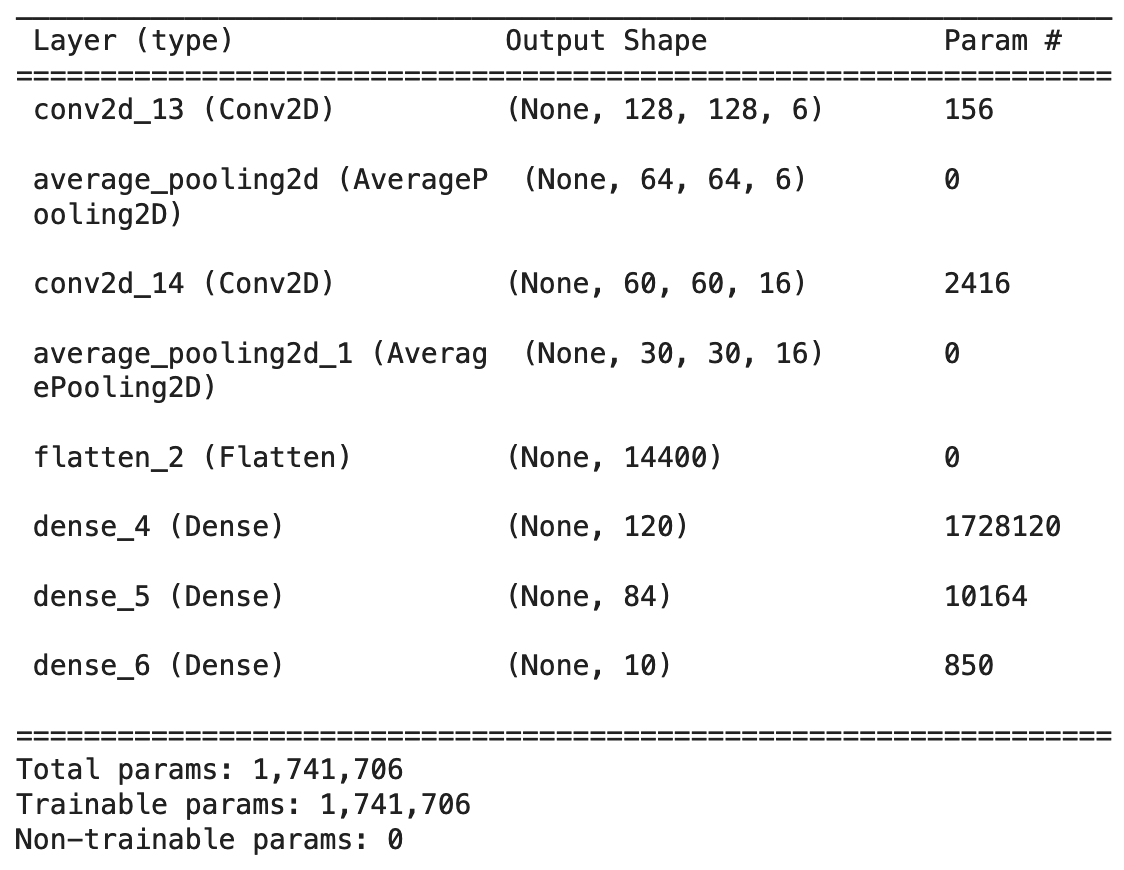
\includegraphics[width=0.48\textwidth]{Images/lenet_summary.png}
    \caption{LeNet Summary}
    \label{fig:lenet_summary}
\end{figure}
You can see the model summaries from figure \cref{fig:cnn_summary} to \cref{fig:lenet_summary}
 ' to remove this section.
%------------------------------------


\section{Additional Information}
\subsection{Python codes}
All of the data processing and network trainings are done on Cats\_And\_Dogs.ipynb file. In \cref{listing:1} a basic implementation of cross validation can be seen. 
% because I have loaded varioref and cleveref (in that order) varioref has "become clever", and you can
% use \Vref{} in the start of a sentence.



\begin{listing}[!htb]

\inputminted[%
firstline=1, 
lastline=15,
bgcolor=LightGray,
breaklines,
breaksymbolleft={},
breakindent={15pt}
]{python}{Code/Python/kfold.py}

\caption{Basic K-Fold implementation}
\label{listing:1}
\end{listing}

The code from \cref{listing:1} was displayed using a \verb+.py+ file. Since the lines are not numbered in this code example, you can copy and paste the code from the PDF into python without many issues (does however need to correct indents). \par
The way cross folding that is implemented in the notebook is vastly different from what its written on here. This code is just an example for it.\par

\section{Model Summaries}
\begin{figure}
    \centering
    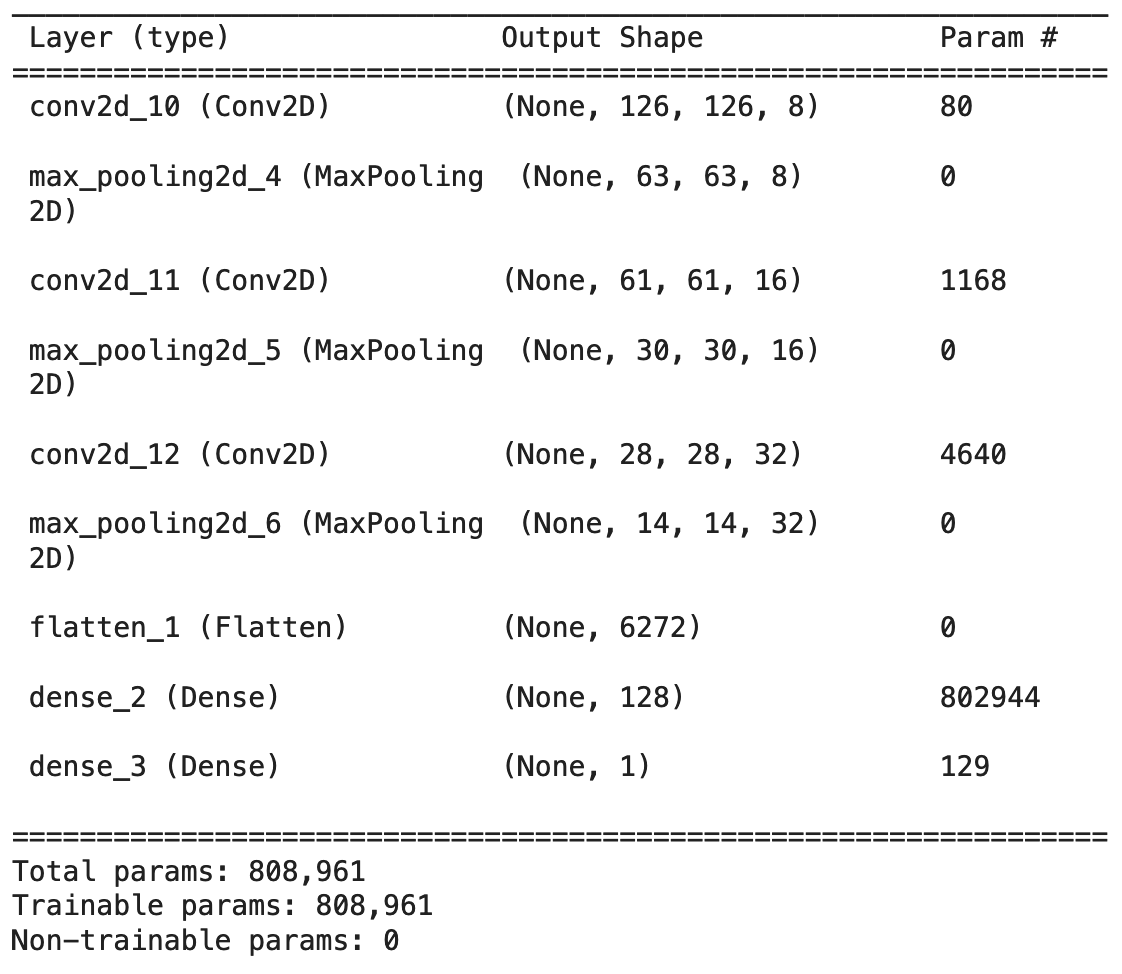
\includegraphics[width=0.48\textwidth]{Images/cnn_summary.png}
    \caption{CNN Summary}
    \label{fig:cnn_summary}
\end{figure}
\begin{figure}
    \centering
    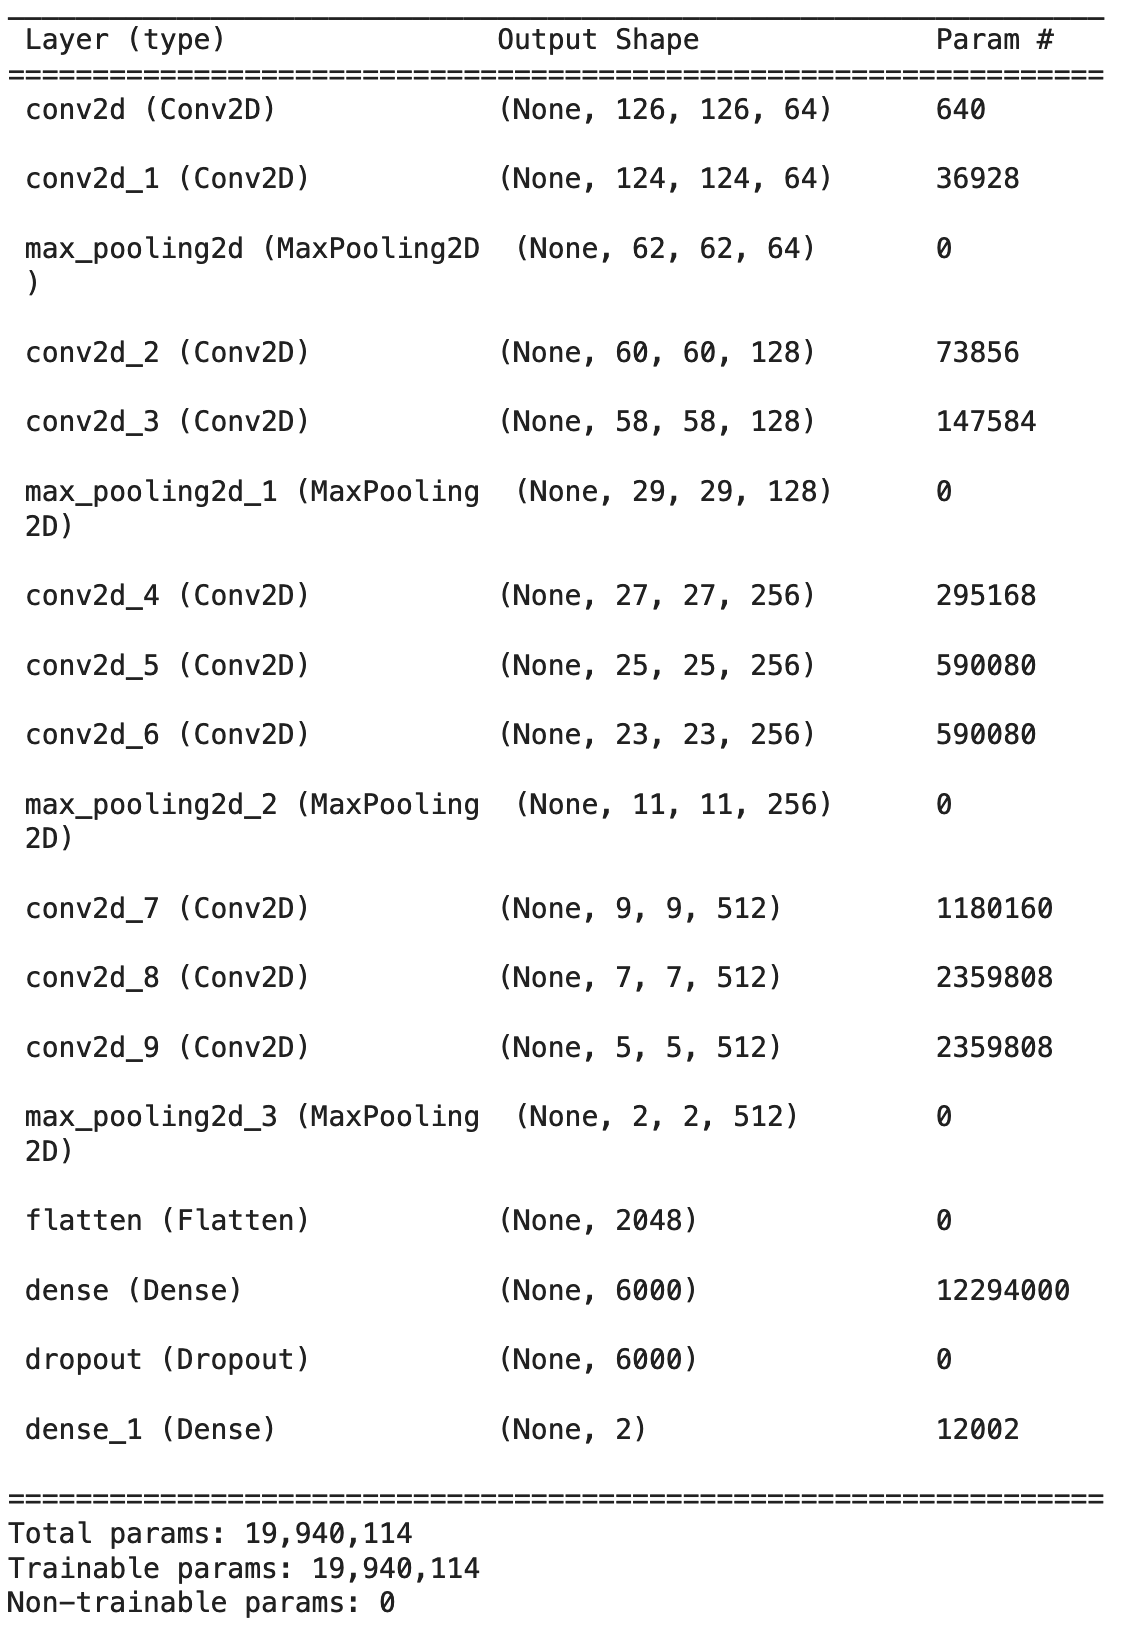
\includegraphics[width=0.48\textwidth]{Images/vgg13_summary.png}
    \caption{VGG13 Summary}
    \label{fig:vgg13_summary}
\end{figure}
\begin{figure}
    \centering
    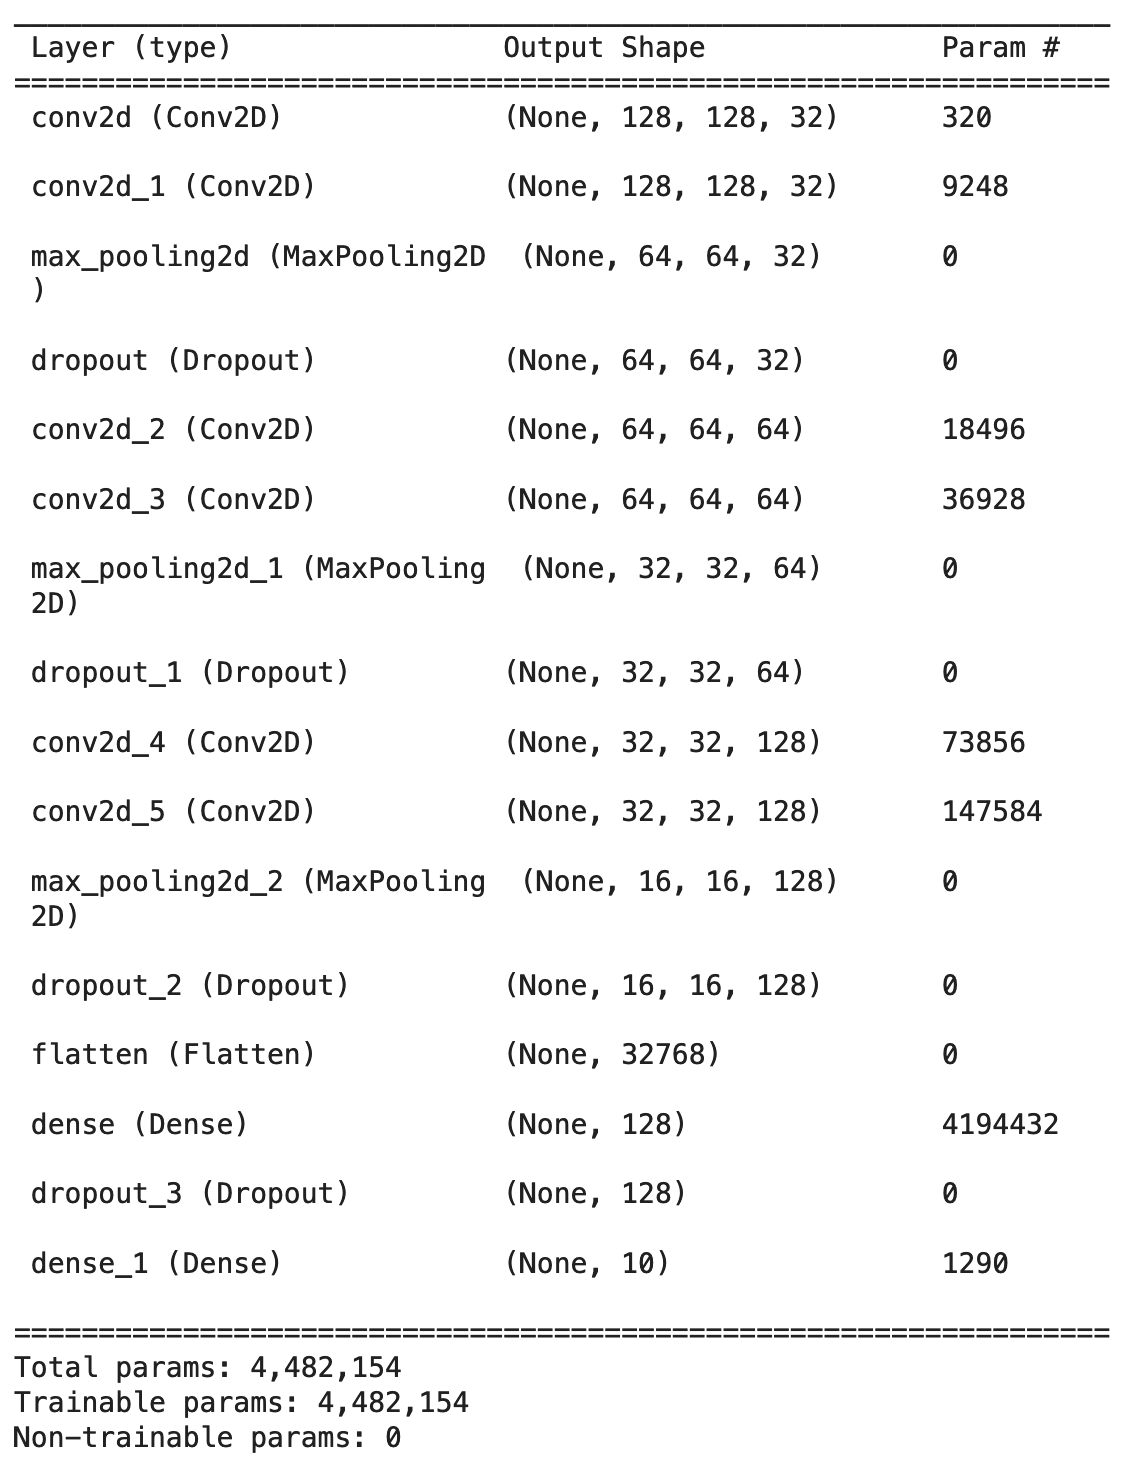
\includegraphics[width=0.48\textwidth]{Images/vgg3_summary.png}
    \caption{VGG3 Summary}
    \label{fig:vgg3_summary}
\end{figure}
\begin{figure}
    \centering
    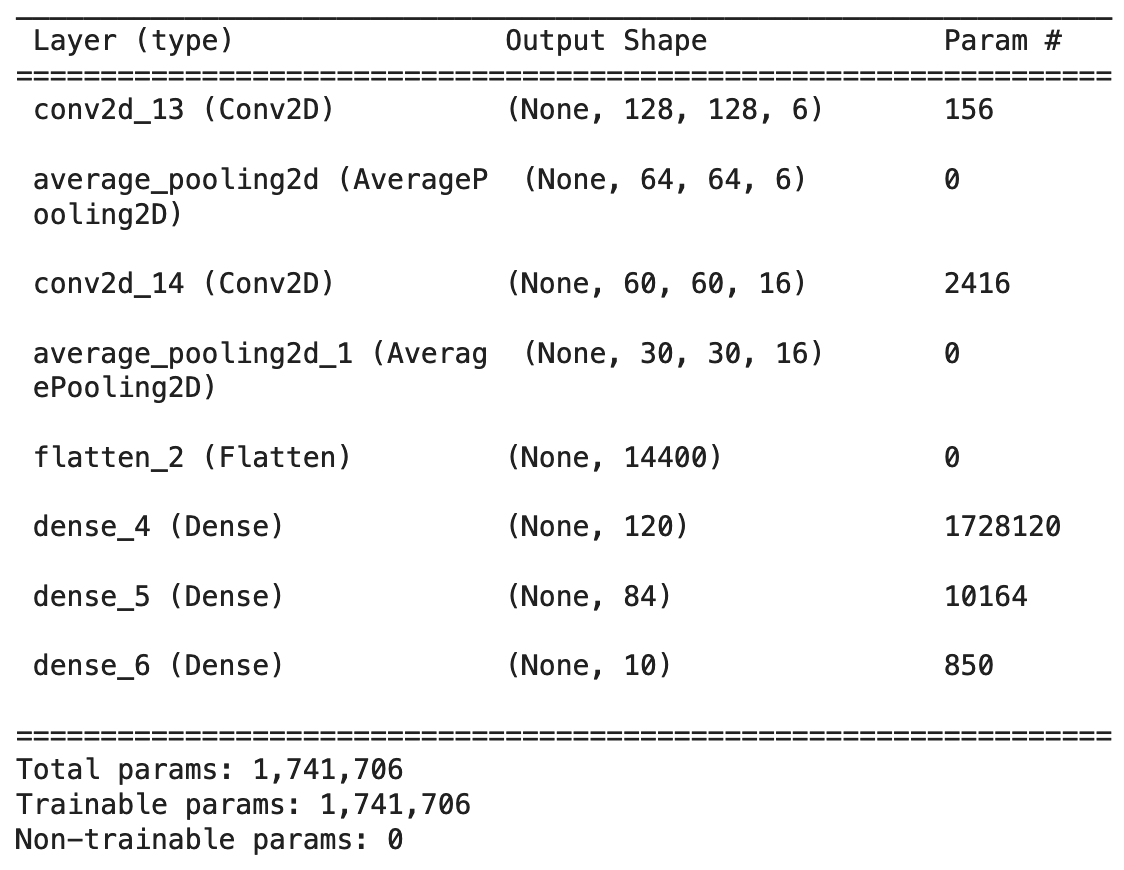
\includegraphics[width=0.48\textwidth]{Images/lenet_summary.png}
    \caption{LeNet Summary}
    \label{fig:lenet_summary}
\end{figure}
You can see the model summaries from figure \cref{fig:cnn_summary} to \cref{fig:lenet_summary}
 ' to remove this section.
%------------------------------------


\section{Additional Information}
\subsection{Python codes}
All of the data processing and network trainings are done on Cats\_And\_Dogs.ipynb file. In \cref{listing:1} a basic implementation of cross validation can be seen. 
% because I have loaded varioref and cleveref (in that order) varioref has "become clever", and you can
% use \Vref{} in the start of a sentence.



\begin{listing}[!htb]

\inputminted[%
firstline=1, 
lastline=15,
bgcolor=LightGray,
breaklines,
breaksymbolleft={},
breakindent={15pt}
]{python}{Code/Python/kfold.py}

\caption{Basic K-Fold implementation}
\label{listing:1}
\end{listing}

The code from \cref{listing:1} was displayed using a \verb+.py+ file. Since the lines are not numbered in this code example, you can copy and paste the code from the PDF into python without many issues (does however need to correct indents). \par
The way cross folding that is implemented in the notebook is vastly different from what its written on here. This code is just an example for it.\par

\section{Model Summaries}
\begin{figure}
    \centering
    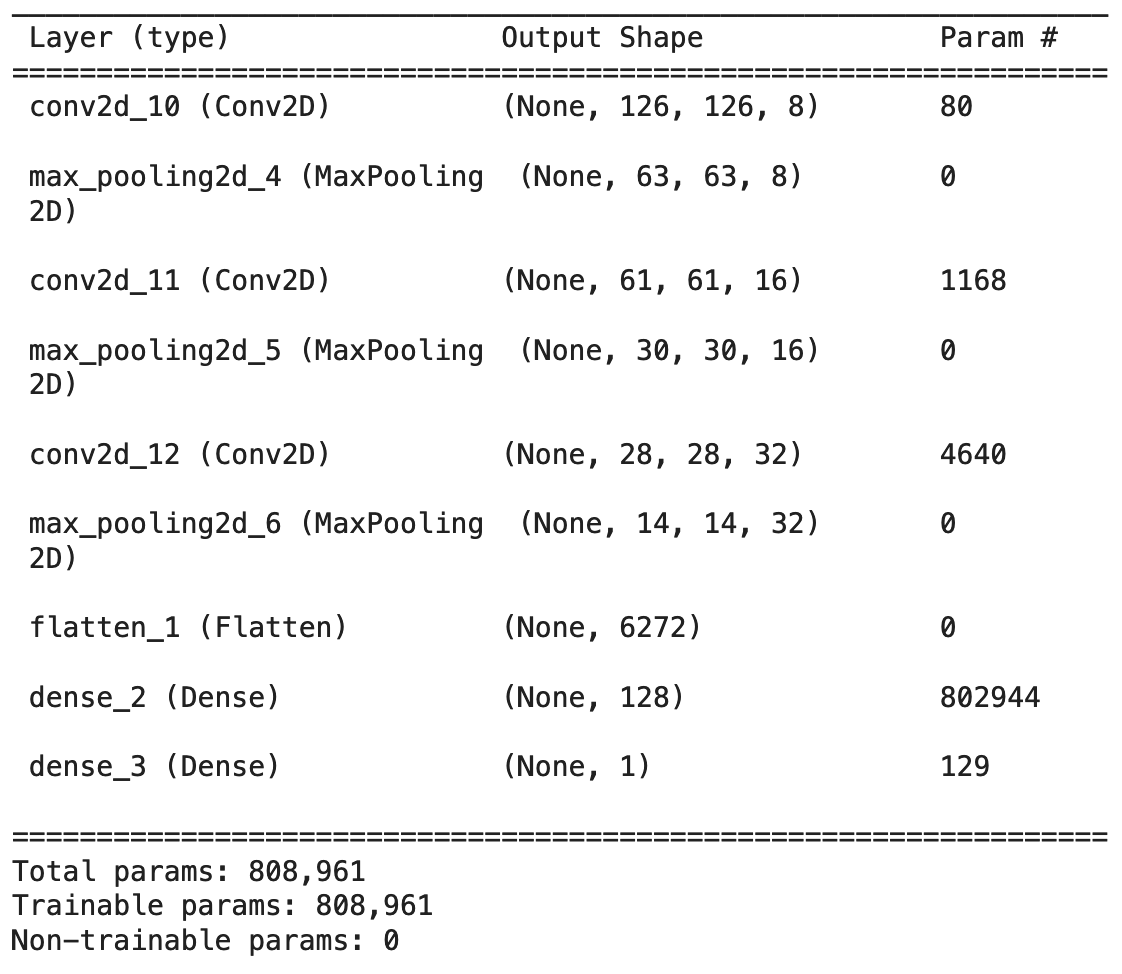
\includegraphics[width=0.48\textwidth]{Images/cnn_summary.png}
    \caption{CNN Summary}
    \label{fig:cnn_summary}
\end{figure}
\begin{figure}
    \centering
    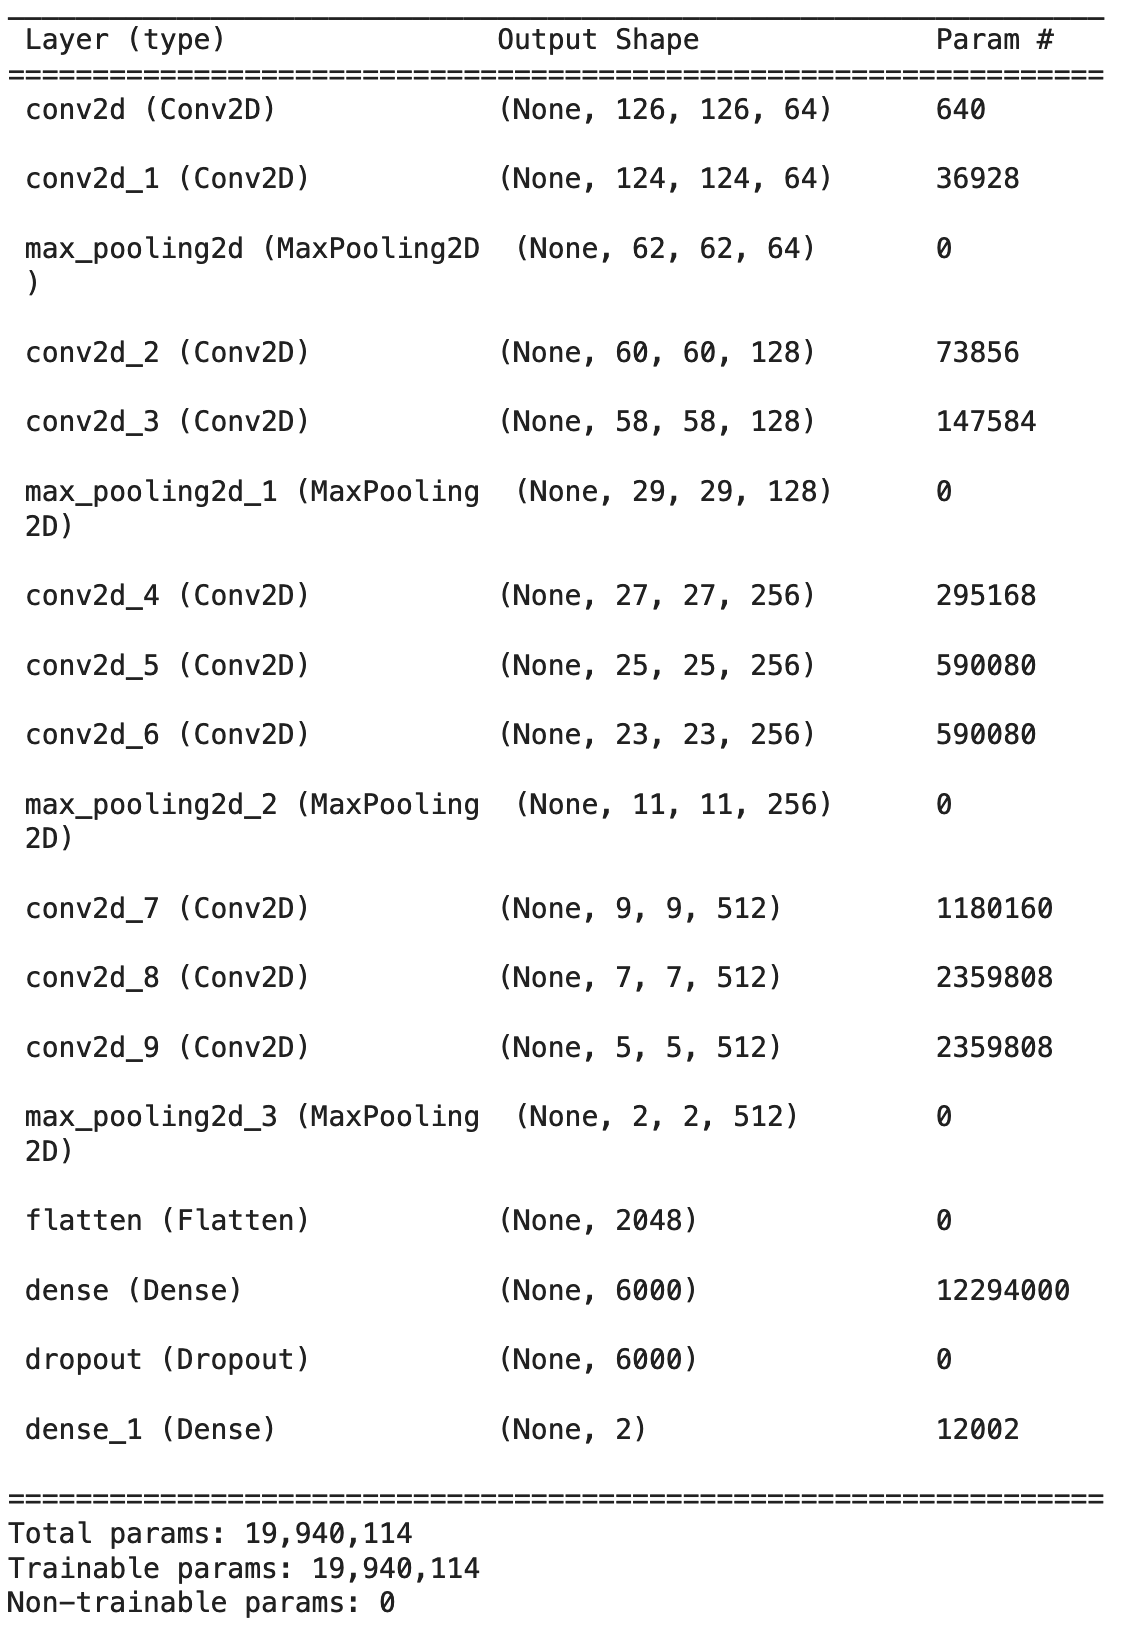
\includegraphics[width=0.48\textwidth]{Images/vgg13_summary.png}
    \caption{VGG13 Summary}
    \label{fig:vgg13_summary}
\end{figure}
\begin{figure}
    \centering
    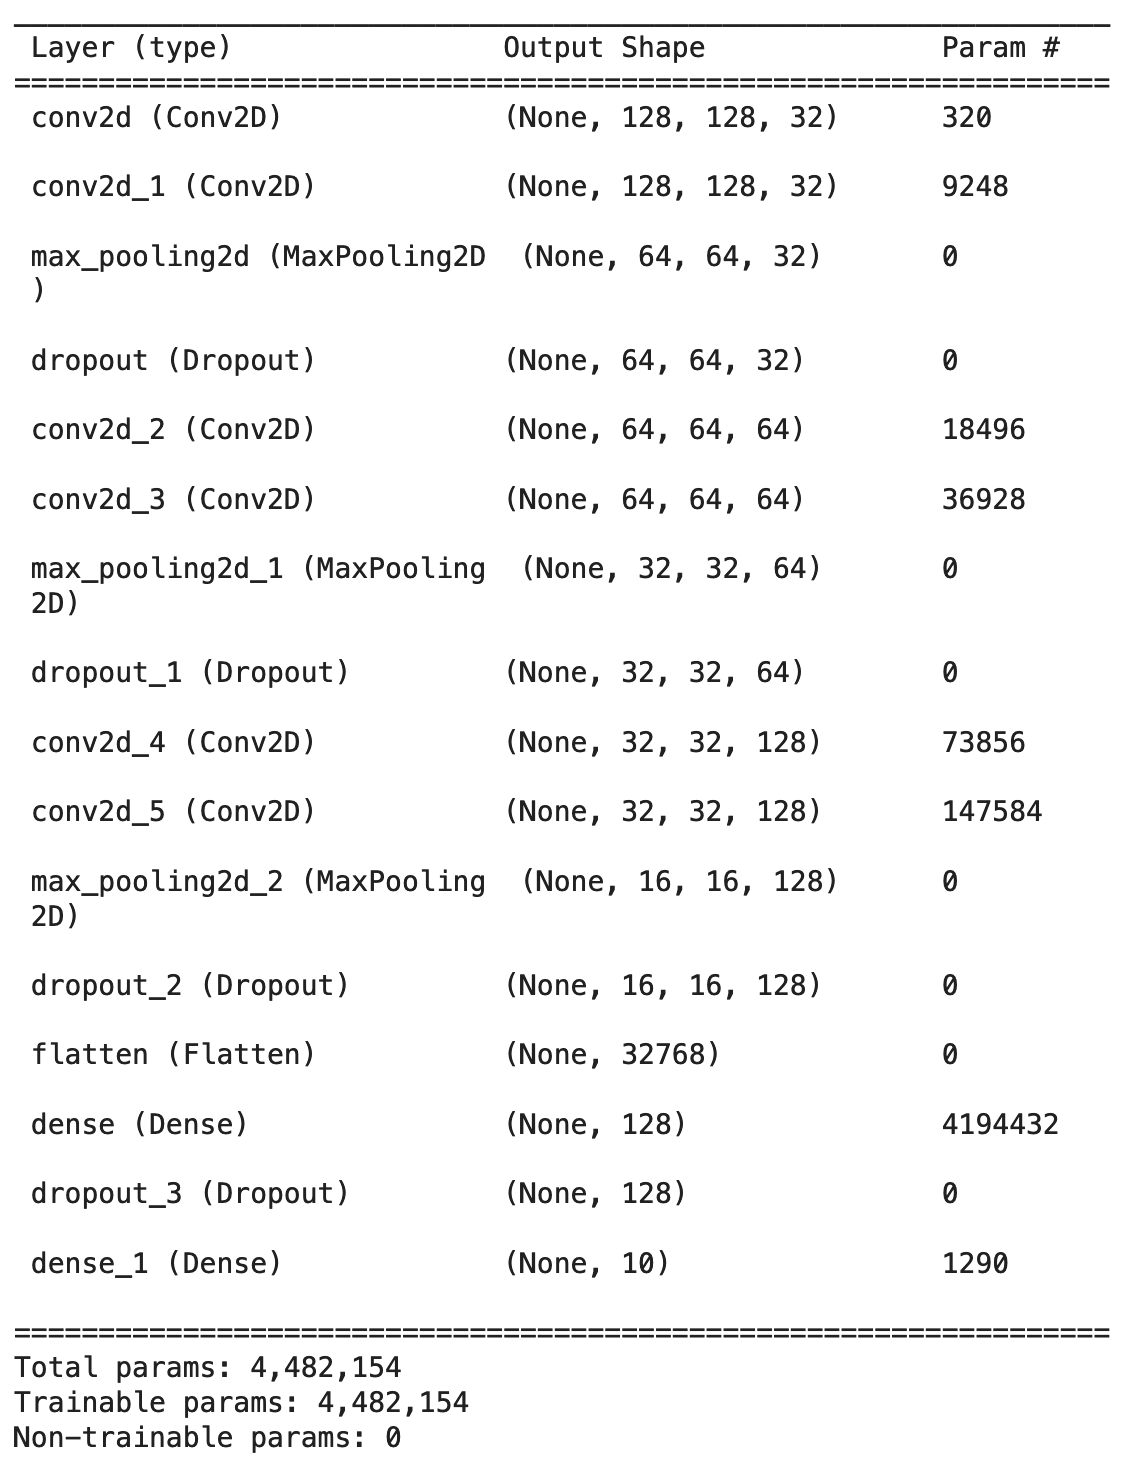
\includegraphics[width=0.48\textwidth]{Images/vgg3_summary.png}
    \caption{VGG3 Summary}
    \label{fig:vgg3_summary}
\end{figure}
\begin{figure}
    \centering
    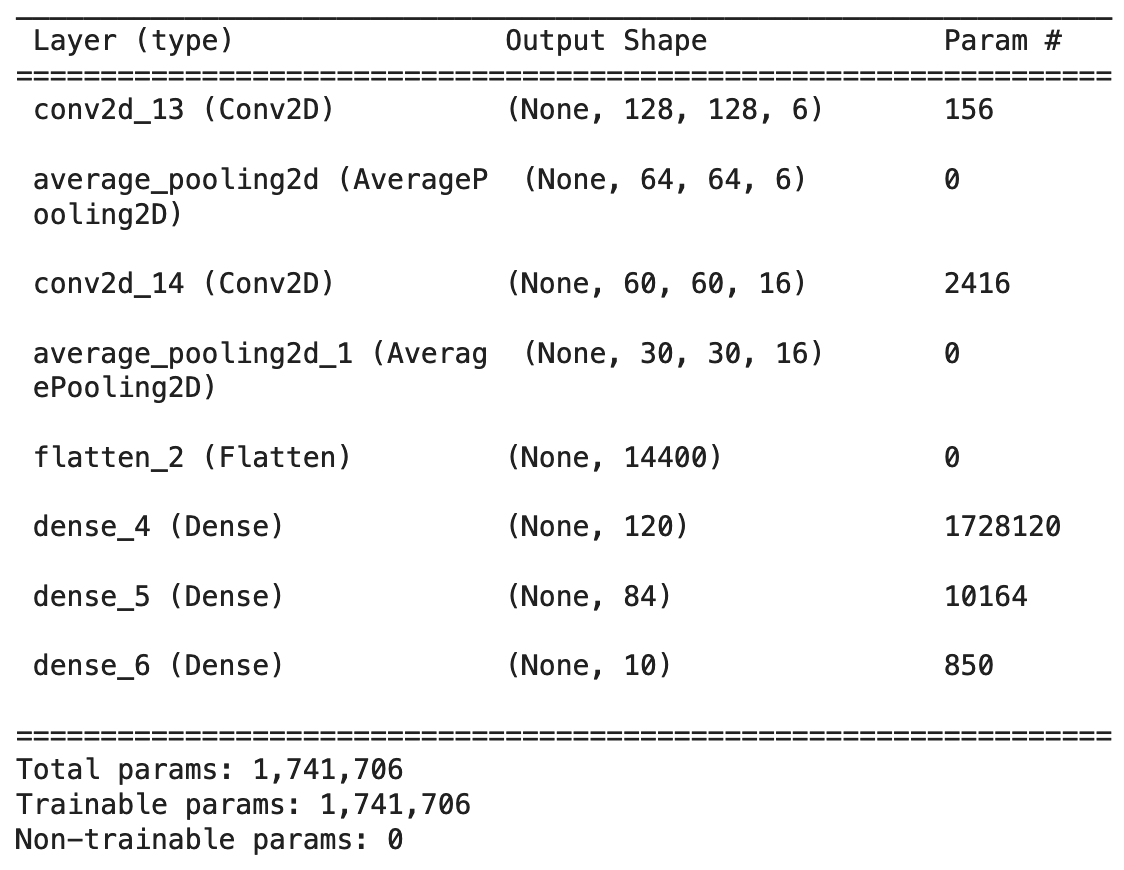
\includegraphics[width=0.48\textwidth]{Images/lenet_summary.png}
    \caption{LeNet Summary}
    \label{fig:lenet_summary}
\end{figure}
You can see the model summaries from figure \cref{fig:cnn_summary} to \cref{fig:lenet_summary}
 ' to remove this section.
%------------------------------------


\section{Additional Information}
\subsection{Python codes}
All of the data processing and network trainings are done on Cats\_And\_Dogs.ipynb file. In \cref{listing:1} a basic implementation of cross validation can be seen. 
% because I have loaded varioref and cleveref (in that order) varioref has "become clever", and you can
% use \Vref{} in the start of a sentence.



\begin{listing}[!htb]

\inputminted[%
firstline=1, 
lastline=15,
bgcolor=LightGray,
breaklines,
breaksymbolleft={},
breakindent={15pt}
]{python}{Code/Python/kfold.py}

\caption{Basic K-Fold implementation}
\label{listing:1}
\end{listing}

The code from \cref{listing:1} was displayed using a \verb+.py+ file. Since the lines are not numbered in this code example, you can copy and paste the code from the PDF into python without many issues (does however need to correct indents). \par
The way cross folding that is implemented in the notebook is vastly different from what its written on here. This code is just an example for it.\par

\section{Model Summaries}
\begin{figure}
    \centering
    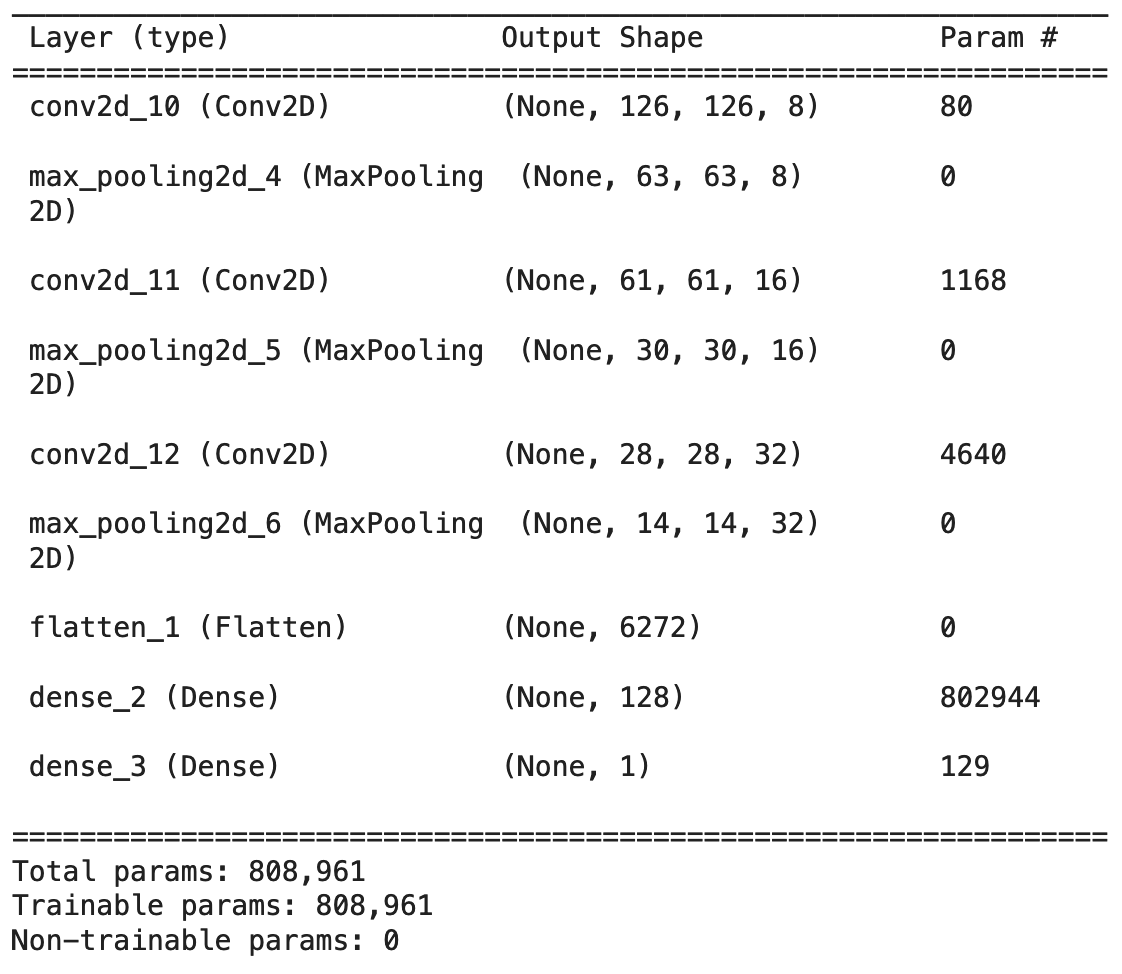
\includegraphics[width=0.48\textwidth]{Images/cnn_summary.png}
    \caption{CNN Summary}
    \label{fig:cnn_summary}
\end{figure}
\begin{figure}
    \centering
    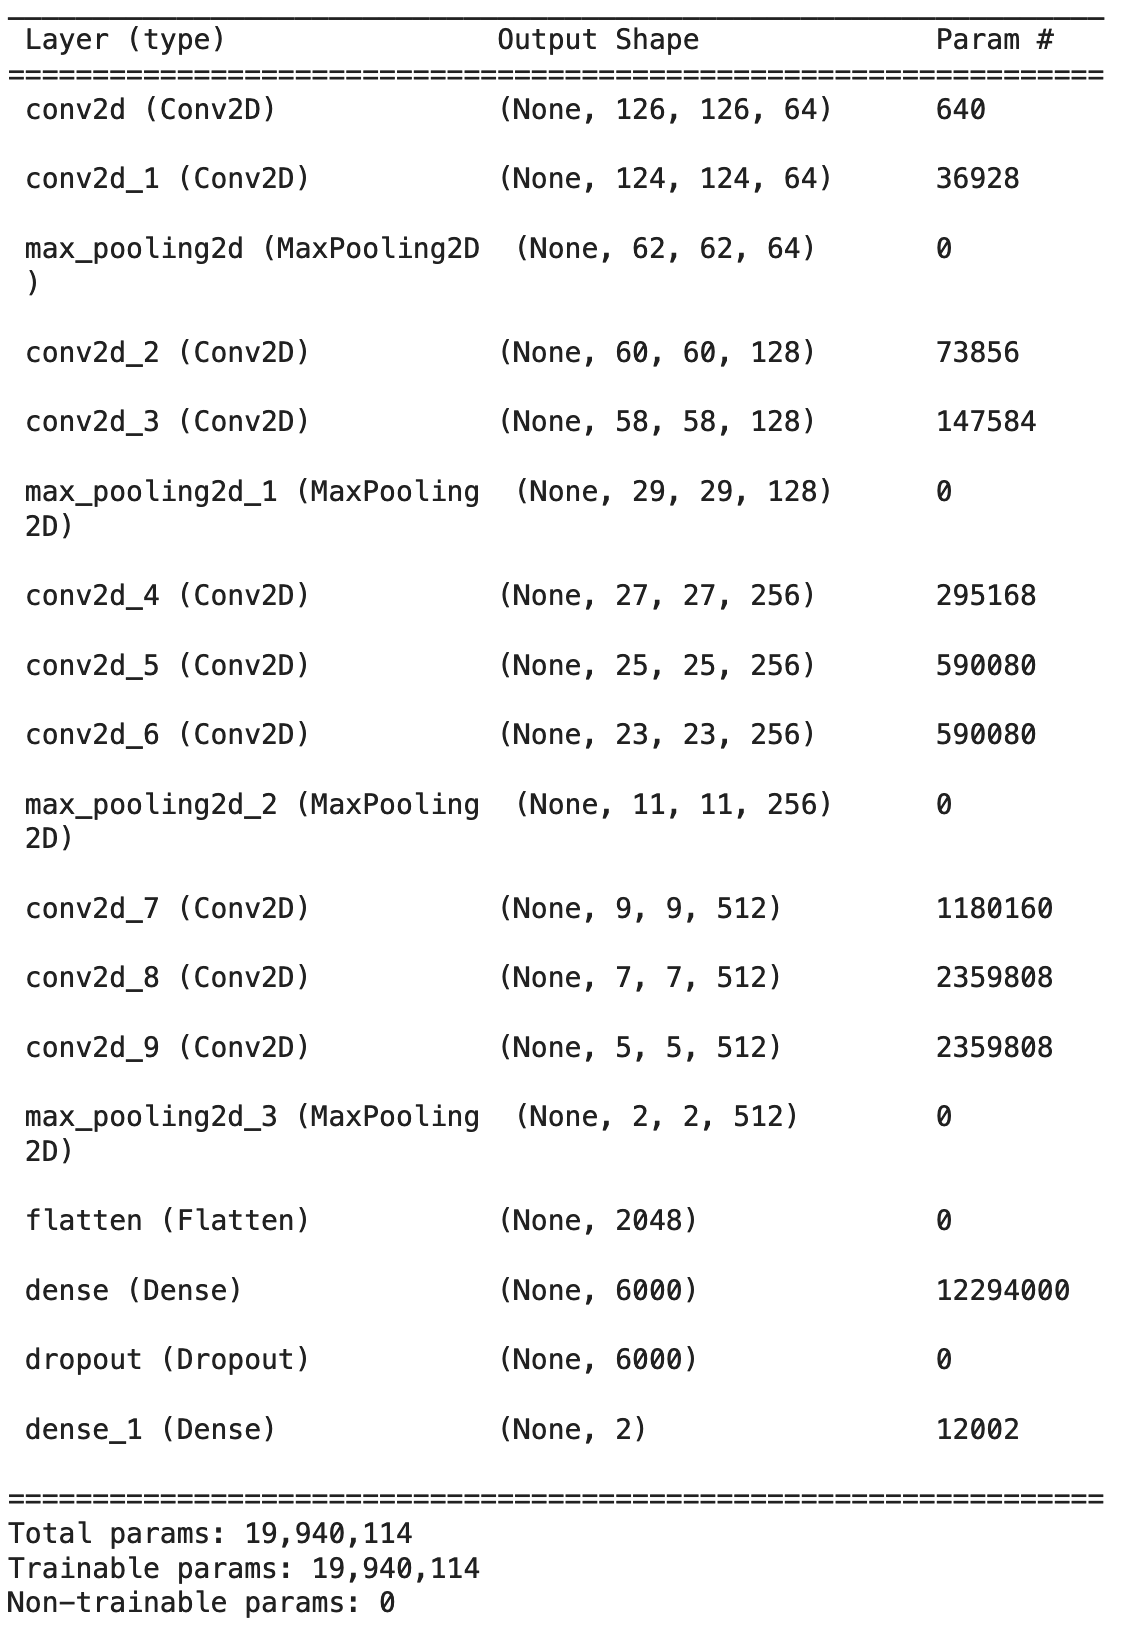
\includegraphics[width=0.48\textwidth]{Images/vgg13_summary.png}
    \caption{VGG13 Summary}
    \label{fig:vgg13_summary}
\end{figure}
\begin{figure}
    \centering
    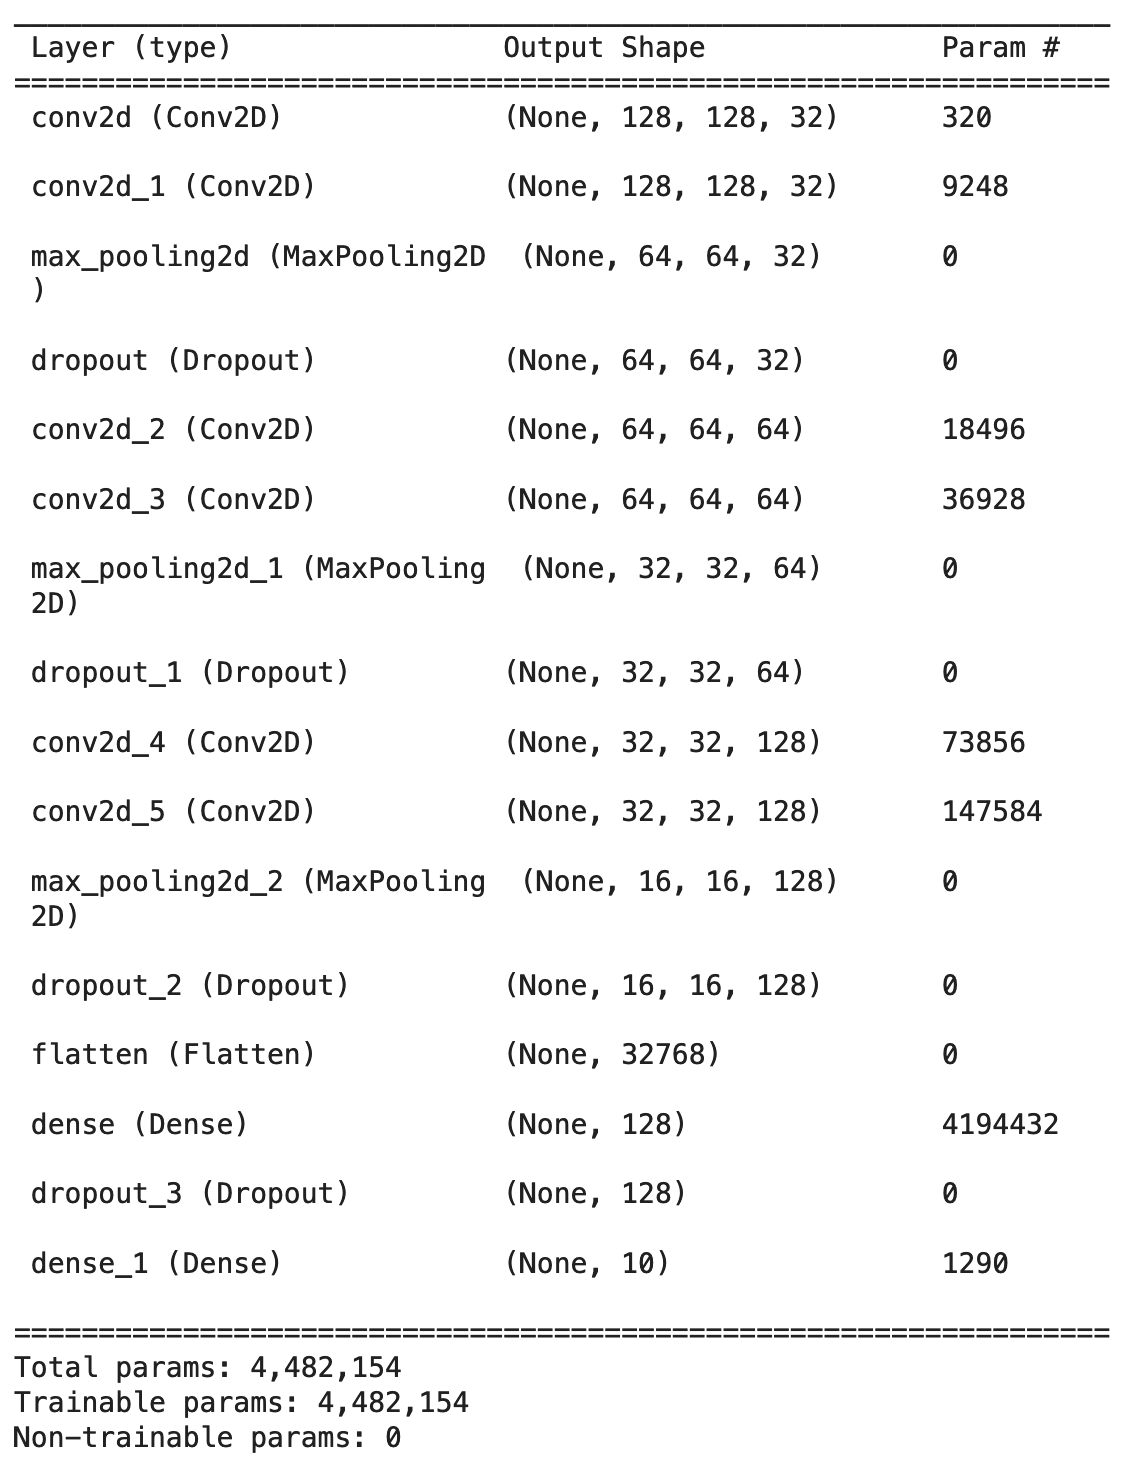
\includegraphics[width=0.48\textwidth]{Images/vgg3_summary.png}
    \caption{VGG3 Summary}
    \label{fig:vgg3_summary}
\end{figure}
\begin{figure}
    \centering
    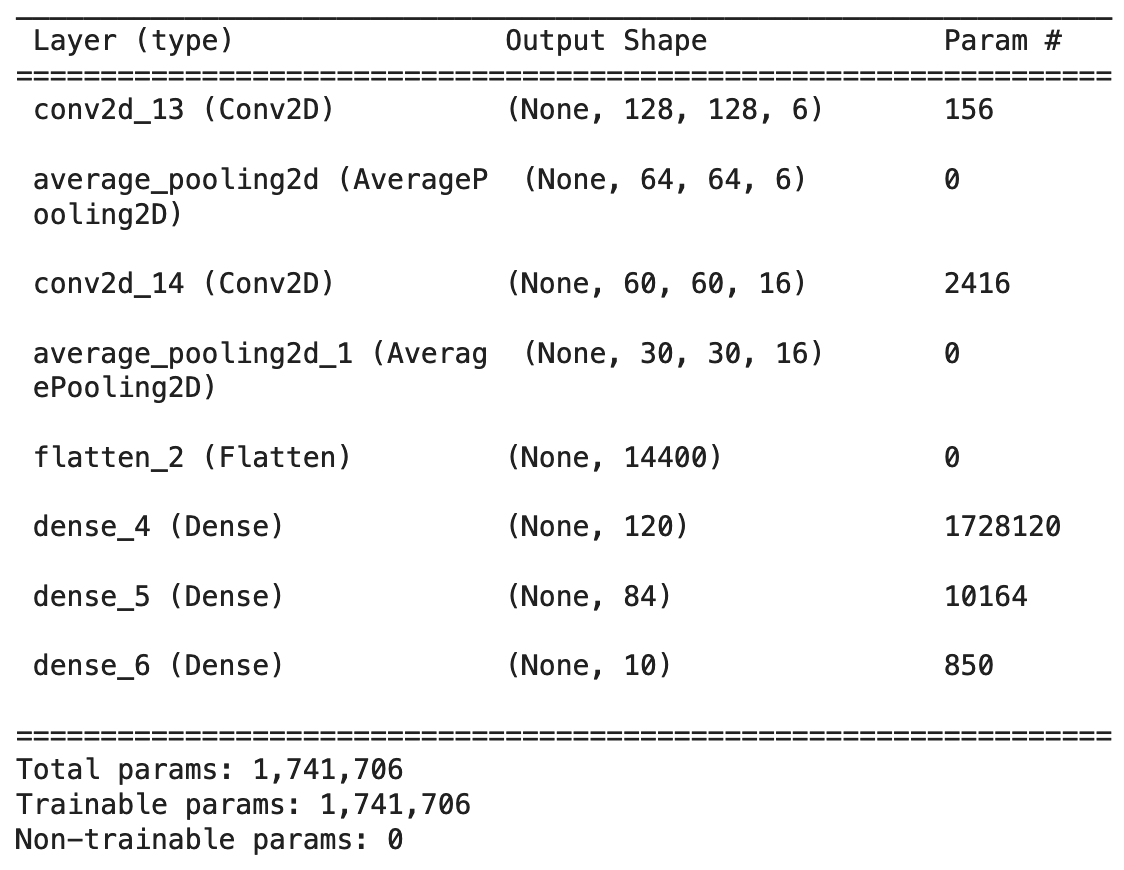
\includegraphics[width=0.48\textwidth]{Images/lenet_summary.png}
    \caption{LeNet Summary}
    \label{fig:lenet_summary}
\end{figure}
You can see the model summaries from figure \cref{fig:cnn_summary} to \cref{fig:lenet_summary}
